\section{Calculadora Medidora de Áreas}

\subsection{Descripción}
La \textit{Calculadora Medidora de Áreas} es una aplicación móvil diseñada para interactuar con un carro controlado remotamente. Su propósito principal es facilitar la medición del área de superficies rectangulares o cuadradas, como mesas, salas, patios, entre otras.

\subsection{Problemática a solucionar}
La intención detrás de este proyecto es simplificar y automatizar la tarea de medir superficies rectangulares. Además, puede ser una solución eficaz en situaciones donde el acceso manual a ciertas áreas es limitado o imposible.

\subsection{Componentes del sistema}
La solución consta de un Arduino, que está conectado a un motor shield, cuatro motores, un receptor Bluetooth, pilas y un power bank. Estos componentes, al interconectarse, dan vida a un carro que obedece instrucciones enviadas desde una aplicación desarrollada en App Inventor.

\begin{figure}[H]
    \centering
    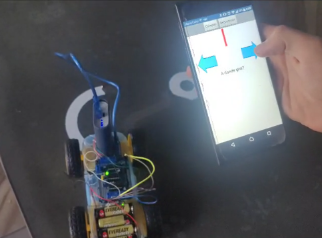
\includegraphics[width=0.7\textwidth]{Figures/0. General/car_controller.png}
    \caption{Control del carro}
    \label{Control del carro}
\end{figure}

\subsection{Motivación}
Más allá de cumplir con un requisito académico, nuestro principal motivador ha sido el deseo intrínseco de aprender y desarrollarnos profesionalmente como ingenieros.

Acá algunas imágenes del proceso de construcción:

\begin{figure}[H]
    \centering
    \begin{subfigure}[b]{0.7\textwidth}
        \centering
        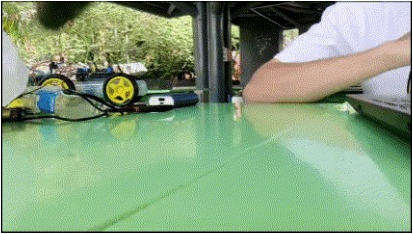
\includegraphics[width=\textwidth]{Figures/0. General/robot_screen.png}
        \caption{``Experiencia es el nombre que todos dan a sus errores.'' ~ Oscar Wilde}
    \end{subfigure}
    \begin{subfigure}[b]{0.6\textwidth}
        \centering
        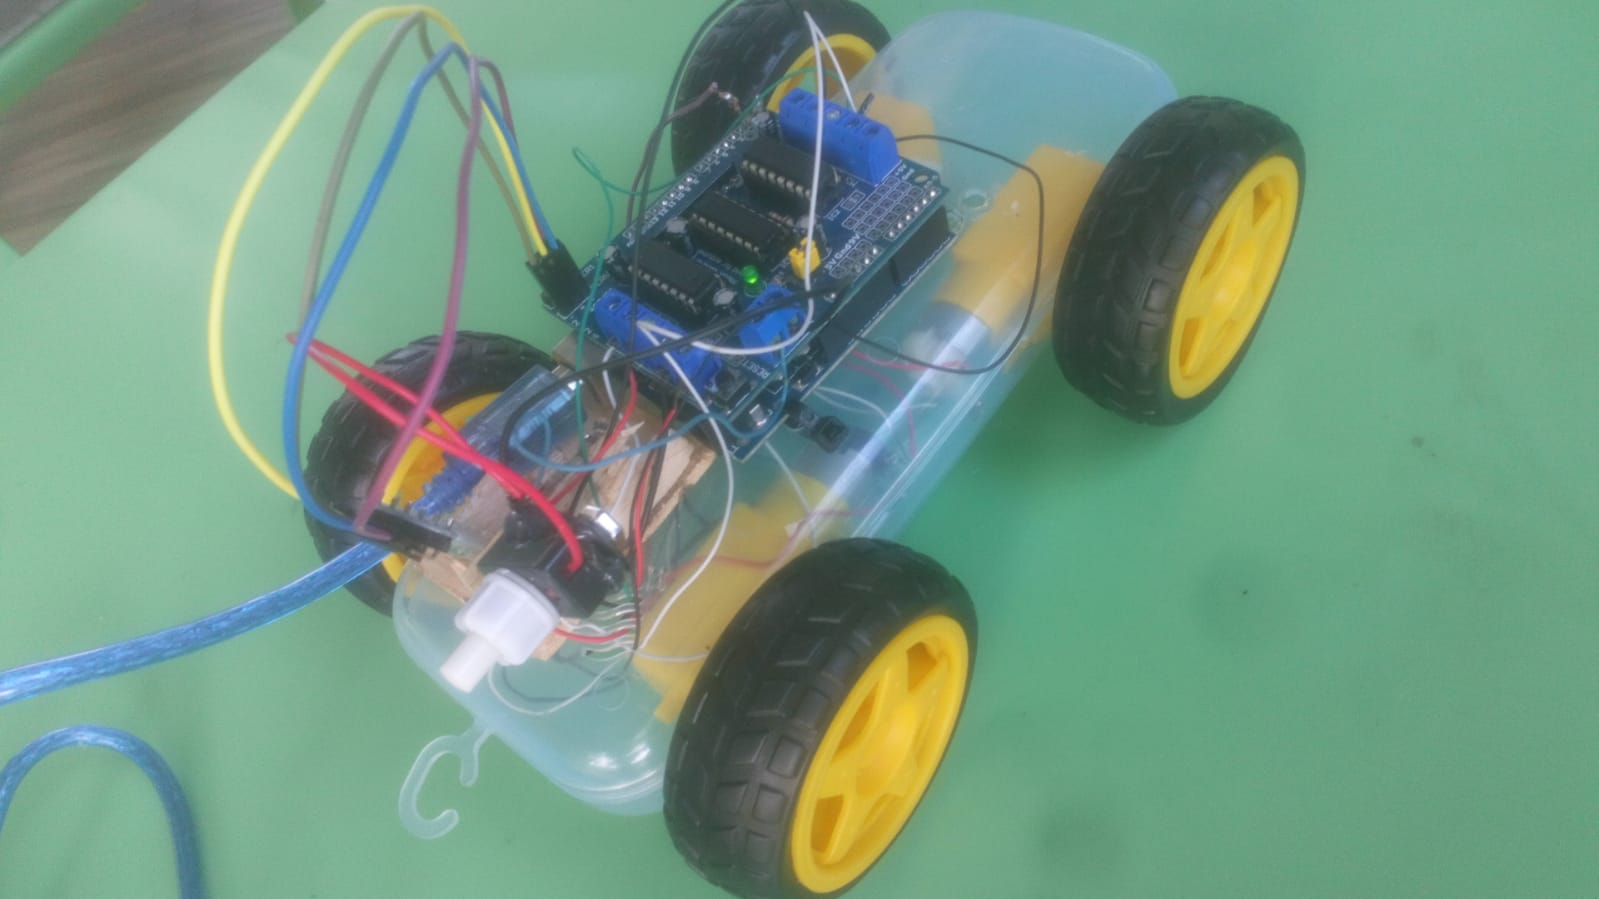
\includegraphics[width=\textwidth]{Figures/0. General/car_controller_2.jpeg}
        \caption{Vista aérea del carro}
    \end{subfigure}
    \begin{subfigure}[b]{0.3\textwidth}
        \centering
        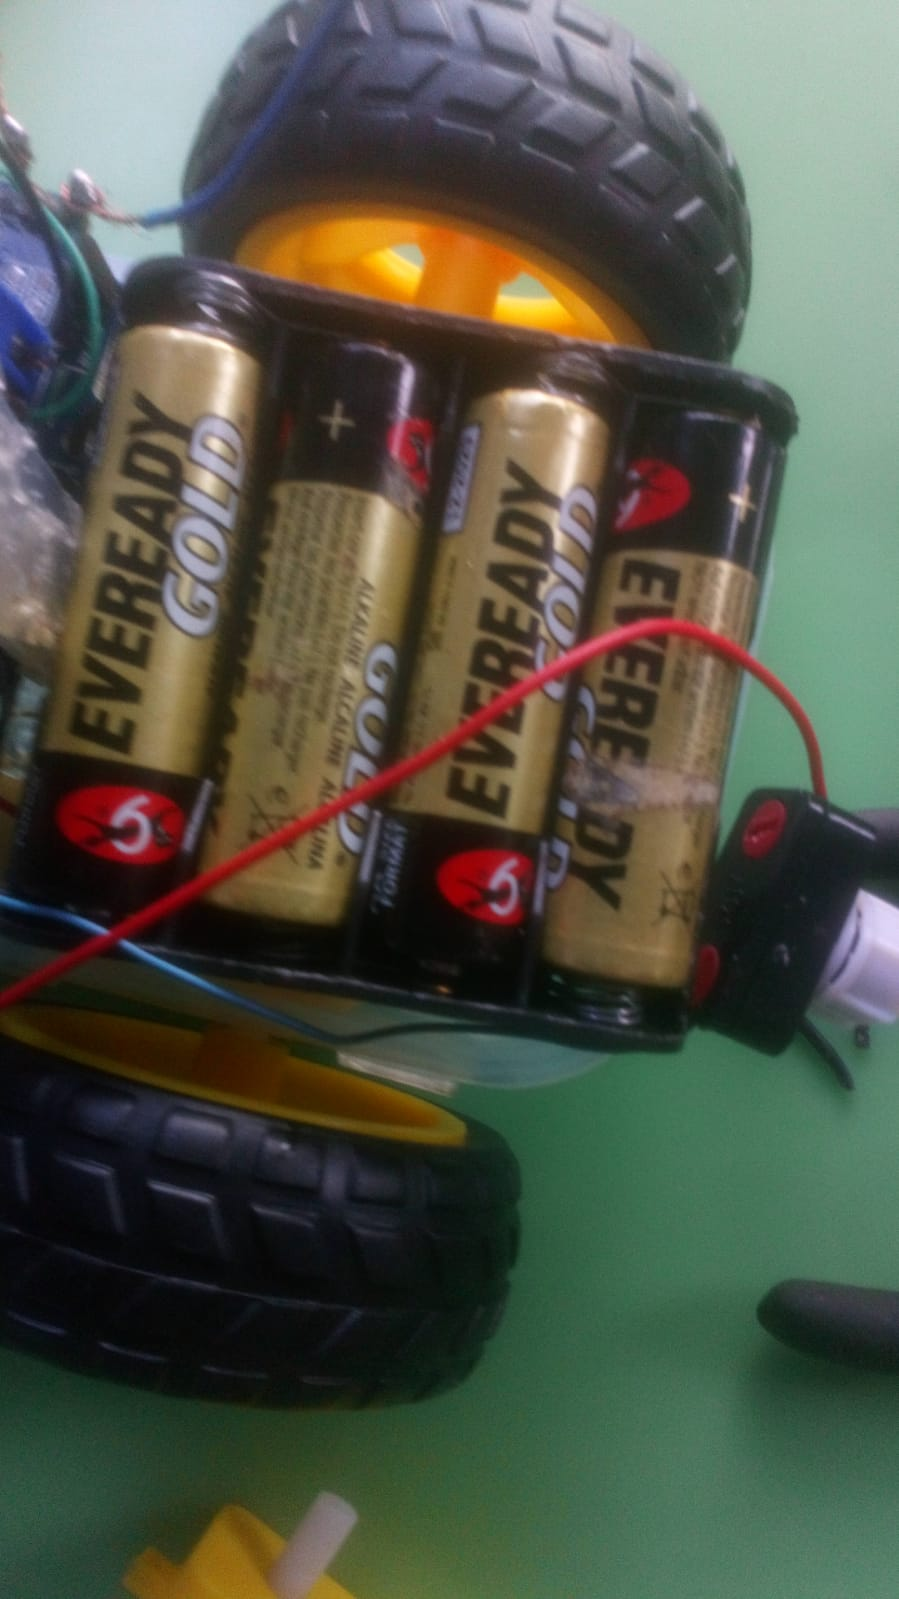
\includegraphics[width=\textwidth]{Figures/0. General/car_controller_1.png}
        \caption{Conexión de la batería}
    \end{subfigure}
    \caption{Instantáneas del proceso}
    \label{fig: tres imágenes}
\end{figure}

\subsection{Funcionamiento}
Para el funcionamiento del Arduino, empleamos dos librerías esenciales: una que facilita el control de los motores mediante el motor shield y otra que gestiona la comunicación con el receptor Bluetooth. El carro se alimenta de una combinación de pilas y un banco de energía, montados sobre un chasis improvisado —curiosamente, una caja de productos de higiene oral— debido a la falta de un chasis comercial disponible.

La aplicación móvil envía señales específicas al Arduino, que a su vez interpreta estas señales para controlar el movimiento del carro. Por ejemplo, al pulsar un botón en la aplicación, se envía una señal que indica al carro avanzar o girar.

\begin{figure}[H]
    \centering
    \begin{subfigure}[b]{0.4\textwidth}
        \centering
        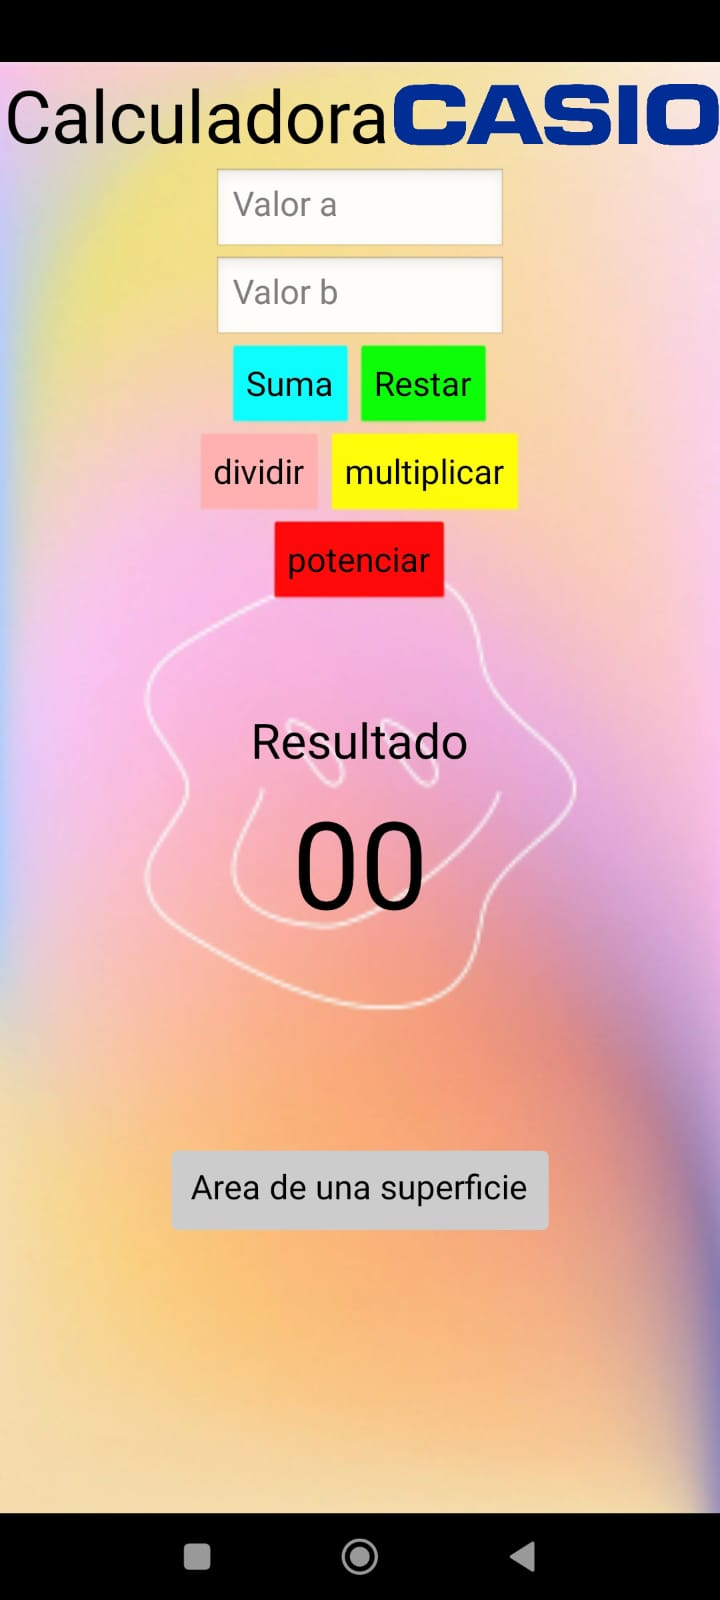
\includegraphics[width=\textwidth]{Figures/0. General/app_screenshot_1.png}
        \caption{Pantalla principal de la aplicación}
    \end{subfigure}
    \begin{subfigure}[b]{0.4\textwidth}
        \centering
        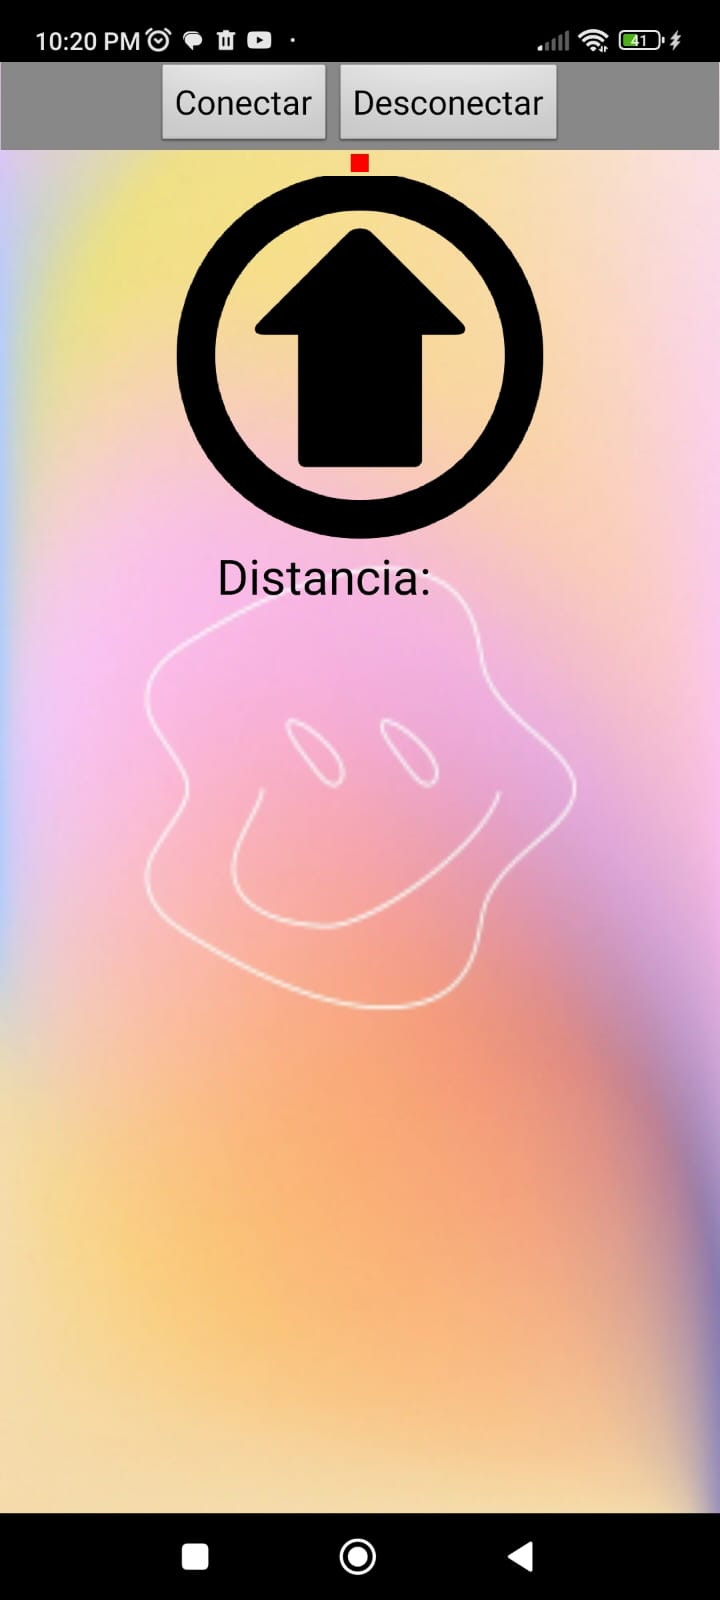
\includegraphics[width=\textwidth]{Figures/0. General/app_screenshot_2.png}
        \caption{Pantalla de medición de distancia}
    \end{subfigure}
    \caption{Interfaz de la aplicación}
\end{figure}

Gracias a que la velocidad del robot es constante, es posible calcular la distancia recorrida al medir el tiempo en movimiento usando la relación:
\[ Distancia = Velocidad \times Tiempo \]
Una vez obtenidas las distancias de dos lados perpendiculares, la aplicación calcula el área mediante el producto de estas medidas. Aunque se realizaron más cálculos y adaptaciones, detallar cada uno excedería la extensión de este documento.

\begin{figure}[H]
    \centering
    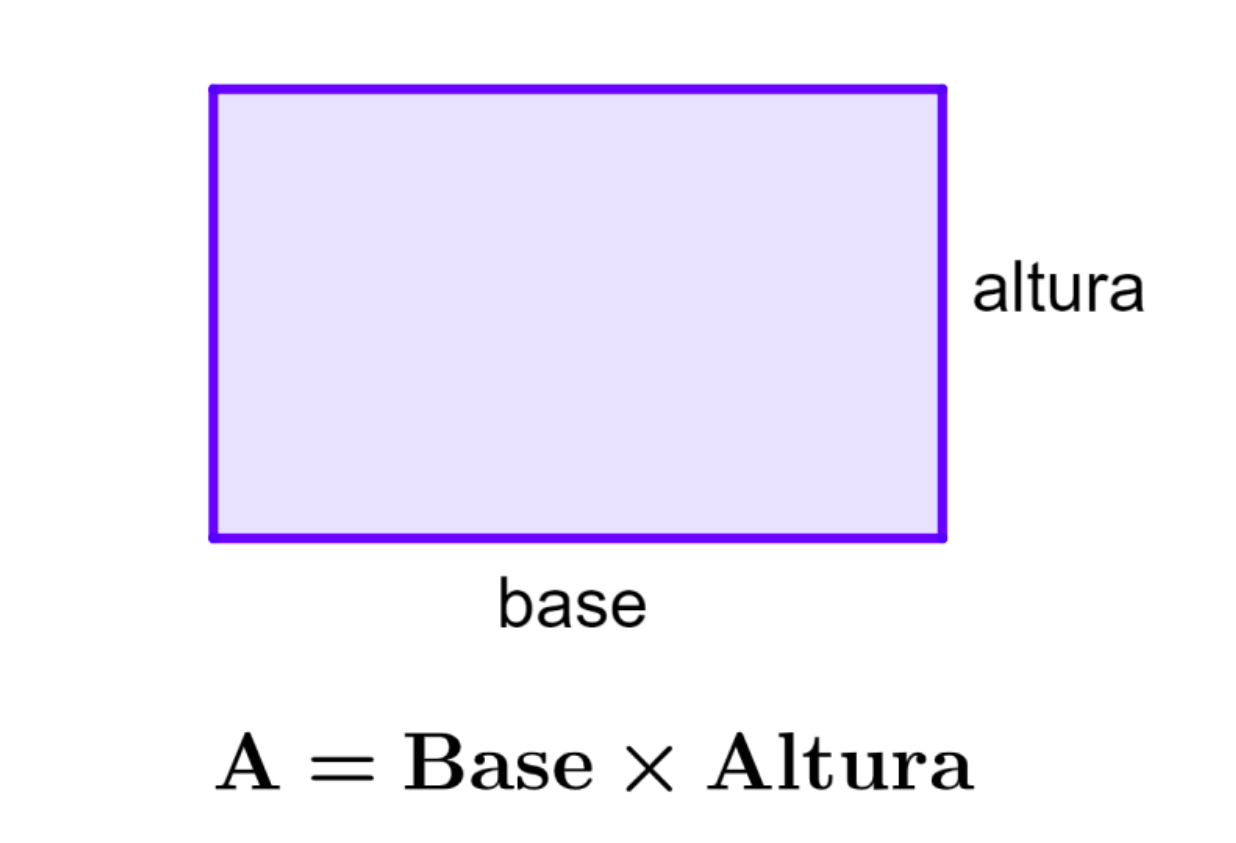
\includegraphics[width=0.4\textwidth]{Figures/0. General/base_altura.png}
    \caption{Cálculo de área: Base x Altura}
\end{figure}

\subsection{Demostración}
Para una comprensión más clara, hemos preparado un video demostrativo de la aplicación, disponible en el siguiente enlace: \url{https://youtu.be/IZjd7NiWPWg}

\begin{figure}[H]
    \centering
    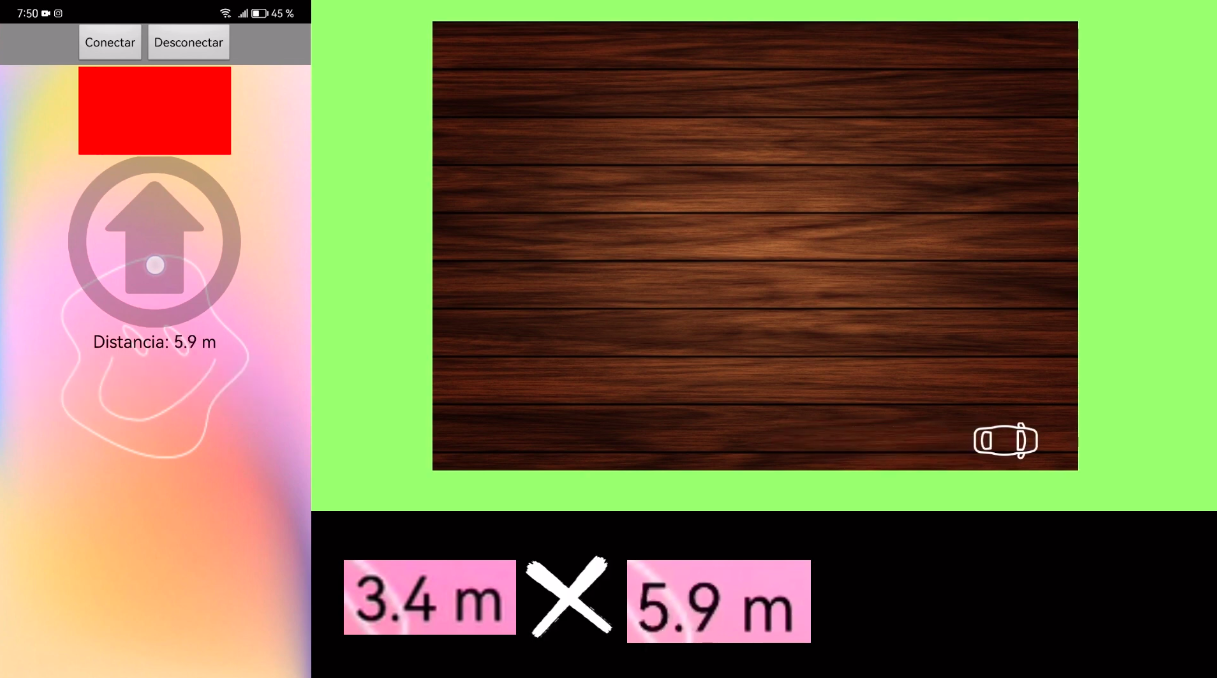
\includegraphics[width=0.7\textwidth]{Figures/0. General/video.png}
    \caption{Vista previa del video demostrativo}
\end{figure}
